In this section we design a framework to collect and analyze addtional data from the point of view of a virtual guest system. 
First, we define the new layers of abstraction in virtual environments.  
Then we identify the virtual resources that require additional information from these layers.
For measuring I/O performance in a virtual guest, we describe the following method to collect and analyze the additional data:
\begin {enumerate}
  \item Identify the relevant performance counters for a resource.
  \item A method to calculate the overhead of virtualization without interference.
  \item A method to analyze performance of a guest machine which may be experiencing degredation from external interference.
\end{enumerate}

% 1 Define the new layers of abstraction virtual environments.
\subsection{Abstraction Layers}
As we have previously stated, a virtual machine could behave unexpectedly due to interference and overhead from virtualization.
Without virtualization, the problem could be in the application, OS, or hardware.  
In a virtual environment, the hypervisor and external guests also need to be considered as a cause of the problem (Table \ref{tab:layers}).  
The hypervisor provides the virtual resources to the guest and controls access to the physical hardware.  
Since the guest machine can only access the hardware through the hypervisor, it will have some performance overhead. 
An external guest machine may also cause interference by competing for resources with other running guest machines.  

\begin{table}[h]
\begin{tabular}{ l p{10cm} }
  Layer & Definition \\
  \hline
  Application & Includes all code and libraries running in user space. \\
  OS & Includes all kernel code and device drivers. \\
  \textbf{Extrenal Guest} & An external virtual system. \\
  \textbf{Hypervisor} & The hypervisor and VMM to manage the guest domains. \\
  Hardare & Physical hardware. \\
  \hline
\end{tabular}
\caption{New layers \emph{Hypervisor} and \emph{External Guest} for virtualizataion}
\label{tab:layers}
\end{table}

% 2 Identify resources which are difficult to measure usage.
\subsection{Resources}
Now we define the virtual resources available to the guest OS and applications.
In a virtual environment, the resources allocated to a guest machine are an abstraction of the physical resources available.  
If a physical resource is used by other layers of virtualization the guest machine will not have complete access to the physical resource.    
Additional information is needed from hypervisor about the physical resource so that the administrator, OS, or application can make better decisions about the availability of the resource. 

\begin{table}[h]
  \begin{tabular}{ l p{10cm} }
    Resource & Definition \\
    \hline
    CPU & The virtual core allocated to the guest \\
    Memory & The virtual RAM allocated to the guest \\
    Disk I/O & The virtual block disk I/O system \\
    Net I/O & The virtual network I/O system \\
    \hline
  \end{tabular}
\caption{Virtual resources which may experience interference from hypervisor or external guest.}
\label{tab:resources}
\end{table}

% 3 Identify the performance counters which can be used to measure I/O performance on a virtual guest machine.
\subsection{Performance Counters}
Performance counters are used by system administrators and developers to show how the resources are utilized and determine if the application is bound by Memory, I/O, or CPU (Table \ref{tab:resources}).  
In other words, adding additional Memory, I/O, or CPU should improve application performance. 
On a Linux OS many of the performance utilities collect statistical data from the /proc filesystem \cite{proc}. 
For example the \emph{sar -d} command will show block device statistics such as transfers/sec, reads/sec, and writes/sec, as well as many other statistics.  
A similar administration GUI, \emph{perfmon.exe}, is available on Microsoft Windows OS which uses an API in the Windows Performance Toolkit \cite{winperf}.  Both of these tools read statistical information from the kernel about the resources and how they are used.

\indent To monitor resource usage of applications and the kernel, administration tools will read these counters over some period of time.  Then it will aggregate and relate the data for that time period.  In some cases, additional inference can be made from different parts of the data.
After aggregating and relating the data, the tool will display the output in some report or graph to show how the system resources are used for that period.
For example to display I/O reads per second every 5 seconds a tool may do the following:
\begin{figure}[h]
\begin{algorithmic}[H]
 \STATE $interval \gets 5$
 \STATE $counter \gets$  Disk Read
 \STATE $pre \gets $ READ $counter$ 
 \LOOP
    \STATE SLEEP $interval$
    \STATE $post \gets$ READ $counter$
    \STATE $result \gets (post - pre)/interval$
    \STATE PRINT  $result$
    \STATE $pre \gets post$ 
 \ENDLOOP
\end{algorithmic}
\caption{Example to display reads per second \emph{rd/s} every 5 seconds.}
\label{alg1}
\end{figure}

\indent For each resource available on a most operating systems, there are many OS level statistics collected about those resources.  It is important to indentify the resources used, and the performance counters for each resource.  Each kernel may have different counters and units of measurement.  A tool that wants to report performance data needs to cleary understand the resource and what events cause the kernel to update the counters.
For our experiments we use I/O and virtual memory statistics, but other statistics could be collected for CPU or network resource usage.

% 4 A method to calculate the overhead and theoritical maximum performance using an offline modeling technique.
\subsection{Virtualization Overhead}
For each virtual resource (Table \ref{tab:resources}) there is a performance cost to making that resource virtualized.  If the guest had direct access to the hardware, at all times, the virtualization cost would be zero.  Since most system calls from the guest kernel needs to go through the hypervisor, we need to account for this additional time, even when the \emph{external guest} layer does not cause interference. 

\indent Several researchers \cite{cherkasova, huber1} have called this cost the \emph{overhead}, and have quantified the overhead for a given configuration.  This research used an offline modeling technique by running a benchmark with and without virtualization.  By calculating the percent difference of these two benchmarks they can calculate the overhead.
The problem with this technique is that physical servers would need to be provisioned for this exercise.  Any configuration changes in hardware or anywhere in the software stack, may require a new test.  

\indent Our method uses a similar approach, but does not actually calculate an actual \emph{cost} for virtualiation.  Our method calculates the percent difference between the usage of the resources in the guest and the usage of resources in the hypervisor.  Since both the guest and hypervisor collects this information it is relatively simple to collect and relate this information.  

\indent We need to calculate the \emph{overhead} before running a guest virtual machine in production, and only needs to be done once.  In large scale datacenters and cloud systems, templates are usually created before virtual machines are used in production.  A template is a complete snapshot image of a virtual machine that has been built and tested to meet some need.  For example a Redhat 6.2 system with an Apache web server may need to be used on several machines.  A system could be built, tuned, and tested for that enviroment and then made into a template.  Future users can deploy a new virtual machine from that template.  We are suggesting to calculate the overhead from virtualization when it is made into a template.  

\indent To calculate the virtualization overhead, create a single virtual machine with dedicated resources on isolated hardware.  
Only one virtual machine should be deployed as we only want to measure overhead from the hypervisor. Next we need to find a test load that will stress the resource (Table \ref{tab:resources}).   
There are many performance benchmarks that can be used \cite{katcher, tikotekar, hplBench}. 
It may be possible to generate a load that will stress I/O, memory, and CPU, but it is best to stress them separately since other interference could mislead results.  
Then place the load on the virtual machine and begin monitoring the performane counters for that resource using the algorithm in Figure \ref{alg1} in BOTH the guest OS and hypervisor. 

\begin{figure}[!h]
  \begin{center}
  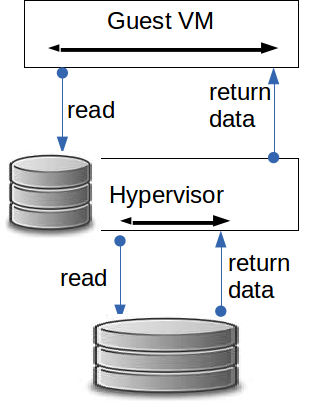
\includegraphics[width=2in]{images/ReadOperation.png}
  \caption{The total time to read from a virtualized disk.  Both the guest and the hypervisor account this statistic in their kernel data.}
  \label{readOp}
  \end{center}
\end{figure}

\indent For a given performance counter and some time interval, we count the hypervisor \emph{count\textsubscript{H}} and the guest \emph{count\textsubscript{G}}. Since we are measuring from the perspective of the guest OS, we want to discover how resources in the guest effect the physical resources.  By monitoring the same resource in both locations, for the same time interval, we can observe the changes as data is sent through the layers of virtualizaion. 

\begin{equation}
  Overhead_V = \frac{count_H - count_G}{count_G} 
\end{equation}

From this equation we can see that there are three cases which can occur:
\begin{enumerate}
	\item \textbf{Overhead} The hypervisor resource counters are greater than the guest. 
	\item \textbf{No Overhead} The hypervisor resource counters are equal to the guest.
	\item \textbf{Negative Overhead} The hypervisor resource counters are less than the guest.
\end{enumerate}
Without knowledge of the hypervisor, one could argue that hypervisor resource counters would be greater than the guest and there would be measurable overhead.  
However, for many of the resource counters we tested we found that there was a negative overhead.  
The hypervisor would optimize the virtual request and not send the same requests to the physical device.

% A method to analyze performance of a guest machine which may be experiencing degredation from external interference.
\subsection{Detecting Interference}
After establishing the overhead for some set of resources and counters we can put the virtual machine into production and run other virtual guests. Now we can try to calculate the interference from external guests.  A naive approach would  simply re-calculate the overhead as in the previous step.  However, this would not (necessarily) describe the interference.  This would only show us that the resource is used by another system.  
It would not tell us if the resource was available to the guest.
We need to collect the same statistics from all guest systems, aggregate those counters, and compare that to the hypervisor.  We need to collect data from all of the layers of virtualization.

\begin{enumerate}
	\item Guest tool requests OS permance counter statistics.
	\item Guest OS forwards request to hypervisor.
	\item Hypervisor forwards request to all guests.
	\item Hypervisor begins monitoring for specified time and waits determined time.
	\item Each Guest responds with individual statistics.
	\item Hypervisor calculates $Overhead_{Vall}$ (Equation 2) of resource used.
	\item Hypervisor returns $Overhead_{Vall}$ to original requestor.
	\item Guest calculates the $Interference$ (Equation 3).
\end{enumerate}

Since the guest has previously calculated $ Overhead_V $ we can use that information to calculate the interference when multiple guests are run concurrently $ Overhead_{Vall}$.  If all \emph{n} guests have been modified to collect and pass information to the hypervisor, each guest can reply with their counters when asked by the hypervisor.  It is important that all guests and the hypervisor start and stop counting concurrently to provide accurate results.  

\[ Count_{Gall} = \sum_{i=1}^n{count_G} \] 
\begin{equation}
Overhead_{Vall} = \frac{count_{Gall} - count_H}{count_{Gall}} 
\label{eq2}
\end{equation}

\indent We can see that when the number of guests machines is 1 (as when we collected the overhead with 1 machine), this is exactly as equation 1.  After the hypervisor calculates the count and overhead for all machines running and passes this information to the original guest, the guest can then calculate the interference.  
The interference from other virtual machines $Interference_V$ is calculated by subtracting the overhead from all guests from the original overhead found without any external interference. 

\begin{equation}
Interference_V = Overhead_{Vall} - Overhead_V
\label{eq3}
\end{equation}

\indent As an example: the userspace tool \emph{iostat} reads disk performance counters in /proc/diskstats and will report transfers, bytes read, and bytes written per second.  If an application was experiencing I/O performance problems this would be a tool an administrator or application developer may monitor.  Without knowing the interference this could be misleading as to the root cause of the problem.  The following example shows a possible output from the perspective of the running guest when experiencing I/O interference from external guest machines.

\begin{figure}[h]
\begin{Verbatim}
Device:  tps    kB_read/s    kB_wrtn/s
sda   577.20     41388.00    148073.00
 virtual I/O interference 22.4%     
\end{Verbatim}
\label{fig:iostat}
\caption{Example:  \emph{iostat} with additional calculated interference.}
\end{figure}

